%%% Local Variables: 
%%% mode: latex
%%% TeX-master: "tellmemore"
%%% End: 

%setup of simulation

\subsection{Overview of Naming Game}
We approach our question through the lens of language evolution. In this case, we view the language in question to consist of the flash patterns of each species, with the caveat that each firefly only has knowledge of its own species' flash signal. 
We model the evolution of this language of firefly flash patterns through a modified minimal naming game, in which the objects to be named are the firefly species, and the words are a fixed length binary sequence.
A naming game broadly conceived proceeds as follows: a population of agents, connected in a certain topology, start with empty memories and follow simple protocols of game rules to achieve consensus on the name of an object. 

In our naming game, the population of agents is a set of individual fireflies.
We view the objects to be named as the firefly species themselves. 
We simplify the problem space by specifying the underlying topology as a complete graph. 
In each time step, either a learning or comparison step is taken for each edge of the graph, as described as follows.

\subsection{Learning and Comparison Steps}
In the full signal naming game, a learning step is executed between fireflies of the same species and a comparison step is executed between fireflies of different species. 
The comparison step of two different species of fireflies is a calculation of a similarity metric with respect to the patterns held in the memory of the fireflies involved. The fireflies keep a running mean of the similarity scores they receive in the comparison step.
The learning step between two fireflies of the same species is a comparison of that running mean. The firefly with the higher (thus worse) score then adopts the pattern of the firefly with the lower score, with a chance of mutation. 
The learning step essentially replicates the better flash pattern with respect to the similarity metric, allowing the population to achieve consensus upon the ``name'' that is the most different from the known flash patterns of other species. 
We introduce a chance of mutation to facilitate the exploration of the pattern space. 

Acknowledging that visual communication in the environment is lossy, we also developed a partial signal naming game in which fireflies converge upon a signal that is not only distinguishable from the known patterns of the other species but also robust to missing bits. 
We designed the comparison step to account for this type of robustness with inspiration from the female responses observed in {\it Photinus} fireflies. 
Instead of simply calculating a similarity metric, one firefly in the pair will send a contiguous subsequence of its pattern. Given this subsequence, the other firefly must make a decision of whether the two are of the same or different species, based upon the similarity of the received subsequence to its own pattern. 
A reward or penalty discounted by the length of the subsequence upon which the decision was made is given to both fireflies based upon the accuracy of the decision. 

Note that the comparison step is taken for all edges in the graph. The learning step is thus only executed in a following round for all pairs of fireflies of the same species. 
This learning step is essentially the same as in the full signal naming game, using the aggregate rewards and penalties to compare and replicate based on the fitness of the flash patterns. 
In this case with positive rewards and negative penalties, a higher aggregate score indicates a higher fitness. 


\subsection{Similarity Metric}
While previous studies (Stanger-Hall and Lloyd 2015) have characterized the periodic flash patterns with four parameters -- flash duration, flash pattern interval, interpulse interval, and female response delay, we relaxed some of those assumptions and chose to characterize flash patterns bit by bit. 
To ensure we capture the periodic nature of the flash signals, we consider the patterns cyclically. That is, we essentially consider the equivalence classes with respect to the permutation cycle $(1 2 3 ... n)$, where $n$ is the fixed length of the flash pattern. 

We propose two different similarity metrics, the first being more straightforward to calculate, while the second better captures our intuitions regarding distinctiveness. 

The first similarity metric counts bit-wise similarity for every possible alignment of the two patterns with respect to the permutation cycle $(1 2 3 ... n)$. That is, for two patterns $p_1, p_2$, we define the similarity score as
\[ \sim (p_1, p_2) = \sum_{i=0}^n \sum_{j=0}^n \mathbb1 \left[p_1 [i+j \mod n], p_2[j] \right] ,\]
where 
\[ \mathbb1 [x,y] = \begin{cases} 1 &\textrm{if } x = y ; \\ 0 &\textrm{otherwise,} \end{cases} \] 
and 
$p[i]$ refers to the $i^{\textrm{th}}$ bit in the pattern $p$, with indexing starting at 0.
We can understand the index $i$ as representing the number of permutation cycles applied to the pattern $p_i$. 

As an example, given two flash sequences of length 5 $[1,0,0,0,0]$ and $[1,0,1,0,0]$, we get a score of 14 using this bit-wise comparison similarity metric. 
If we require at least one bit to be ``on" in the sequence, then the lowest possible score is 5, realized by the two sequences $[1,0,0,0,0]$ and $[1,1,1,1,1]$. Generalizing to sequences of length $n$, the minimum score is thus $n$. 
The highest possible score -- that is, two identical patterns -- is 25, or $n^2$.

The second similarity metric we use simply measures the length of the longest common subsequence. Here, we compare shared subsequences between doubled flash patterns, that is we consider subsequences that are ``wrapped." 
 Mathematically, we can define our second similarity metric as follows,
\[ \sim (p_1, p_2) =  \max _{i \in [0,2n-1], j \in [0,2n-1]} T[i][j], \] 
where {\tiny \[ T[i][j] = \begin{cases} T[i-1][j-1] + 1 &\textrm{if } p_1[i-1 \mod n] = p_2[j-1 \mod n] \\
	0 &\textrm{otherwise.} \end{cases}\]}
	
Revisiting the previous examples, the longest contiguous subsequence shared between $[1,0,0,0,0]$ and $[1,0,1,0,0]$ is $[0,1,0,0]$, giving a similarity score of 4. 
The lowest possible score using this metric is 1, again instantiated in patterns of length 5 by the two sequences $[1,0,0,0,0]$ and $[1,1,1,1,1]$. 
The highest possible score for two identical patterns is 9, or $2n-1$, where $n$ is the length of the pattern. 
We see an immediate difference in range for these two similarity metrics and how they differ in capturing degrees of similarity. 

This second similarity metric can be modified for a partial sequence and is used in the partial signal naming game in order to decide whether a subsequence belongs to the same species. 
That is, we find the longest common substring between the full pattern of one firefly and the subpattern of the other and use that length divided by the length of the subsequence with a constant decision threshold. 
Specifically, et $p_2$ be a partial sequence with length $m$. Then, the decision score is 
\[ d(p_1, p_2) = \max _{i \in [0,2n-1], j \in [0,m]} T[i][j], \] 
where {\tiny \[ T[i][j] = \begin{cases} T[i-1][j-1] + 1 &\textrm{if } p_1[i-1 \mod n] = p_2[j-1] \\
	0 &\textrm{otherwise.} \end{cases}\]}
We note that we ``wrap" the full pattern but do not do so for the partial pattern. 

\subsection{Risk of Flashing -- Score Discounting}
To address the physiological cost of producing a flash and the predation risk of flashing, we discount scores with respect to the number of flashes in the signal in order to select towards more limited time spent flashing. 
In the full signal naming game, in which a lower score indicates a fitter flash pattern, the score that is compared during the learning step is multiplied by the number of flashes divided by 3. Specifically, the similarity score between two patterns $p_1$ and $p_2$ from the perspective of the firefly with pattern $p_1$ is, \[ \textrm{score}(p_1, p_2) = \frac{\sum_{i = 1}^{n} p_1[i]}{3} \sim(p_1, p_2).\]

Conversely, in the partial signal naming game, in which a higher aggregate reward indicates more success in the comparison step, the reward used in the learning step is divided by the total number of flashes in the pattern. 
%the similarity score between two patterns $p_1$ and $p_2$ from the perspective of the firefly with pattern $p_1$ is, 
%\[ \textrm{score}(p_1, p_2) = \frac{\sim(p_1, p_2)}{\sum_{i = 1}^{n} p_1[i]}. \]

%\subsection{Mutation Methods}

\begin{figure}[h]
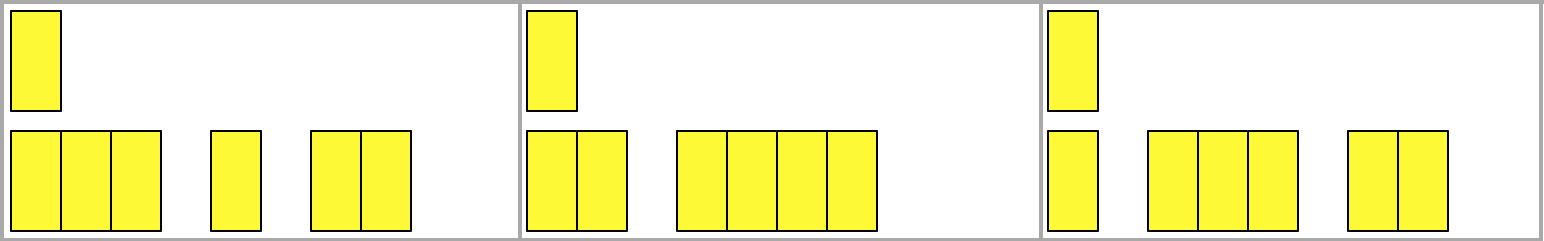
\includegraphics[width = \columnwidth]{./pictures/2_lcs_one/all.png}
\caption{Top results for 2 species full pattern naming game, with similarity scores from left to right of 3, 4, and 4.}
\end{figure} 

\begin{figure}[h]
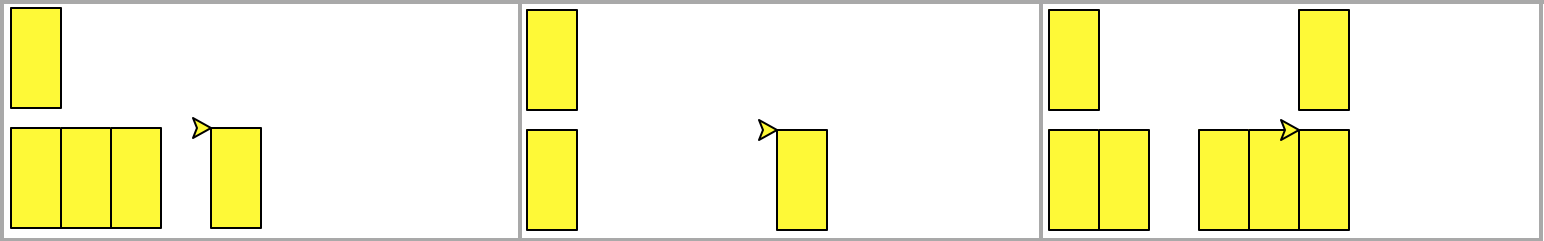
\includegraphics[width = \columnwidth]{./pictures/2_lcs_two/all.png}
\caption{Top results for 2 species partial pattern naming game, with similarity scores from left to right of 7, 9 and 12.}
\end{figure} 

\begin{figure}[h]
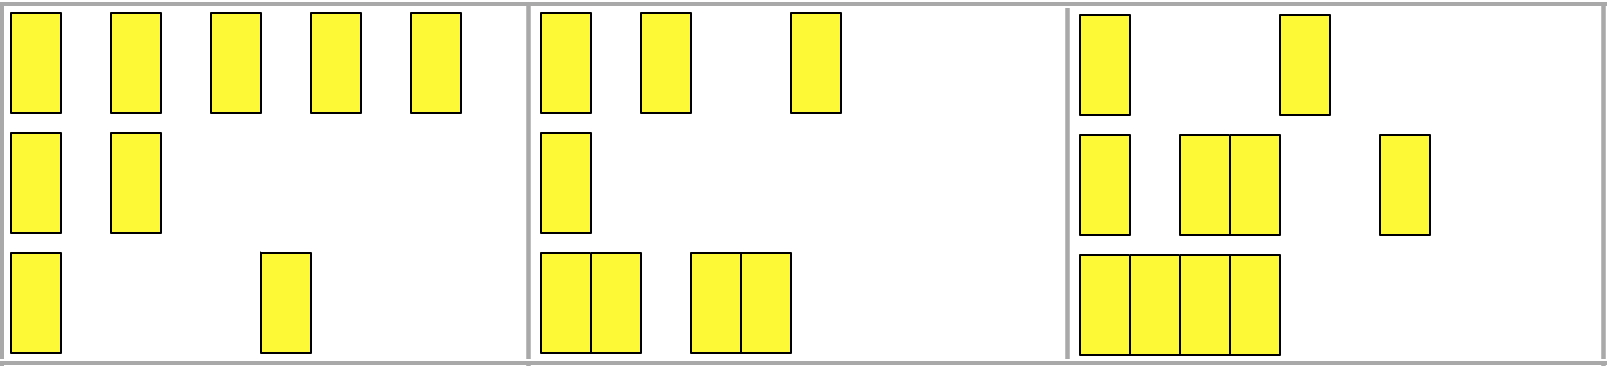
\includegraphics[width = \columnwidth]{./pictures/3_lcs_one/all.png}
\caption{Top results for 3 species full pattern naming game, with similarity scores from left to right of 17.3, 21.7, and 24.}
\end{figure} 

\begin{figure}[h]
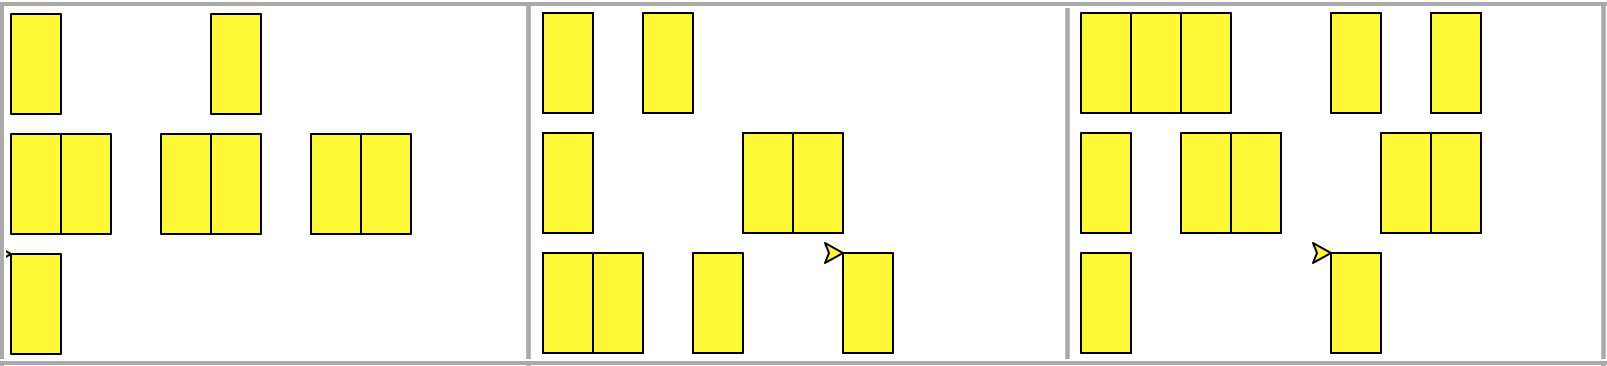
\includegraphics[width = \columnwidth]{./pictures/3_lcs_two/all.png}
\caption{Top results for 3 species partial pattern naming game, with similarity scores from left to right of 18, 24.7, and 25 .}
\end{figure} 

\begin{figure}[h]
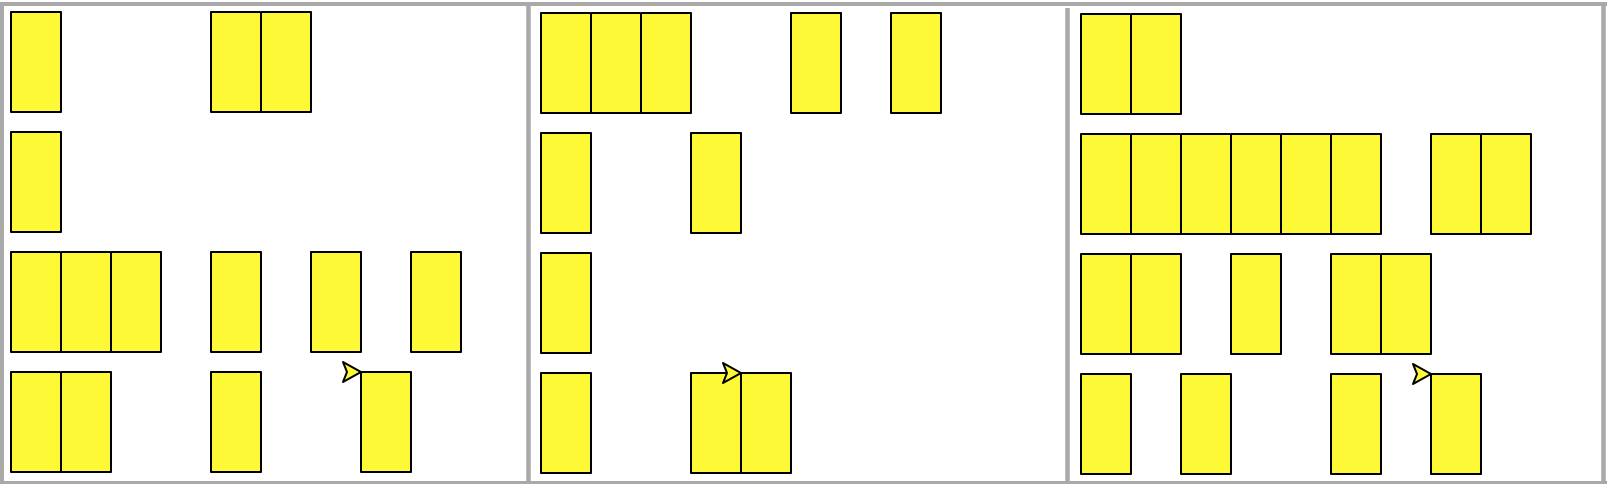
\includegraphics[width = \columnwidth]{./pictures/4_lcs_one/all.png}
\caption{Top results for 4 species full pattern naming game, with similarity scores from left to right of 20.3, 21.3, and 26.3.}
\end{figure} 

\begin{figure}[h]
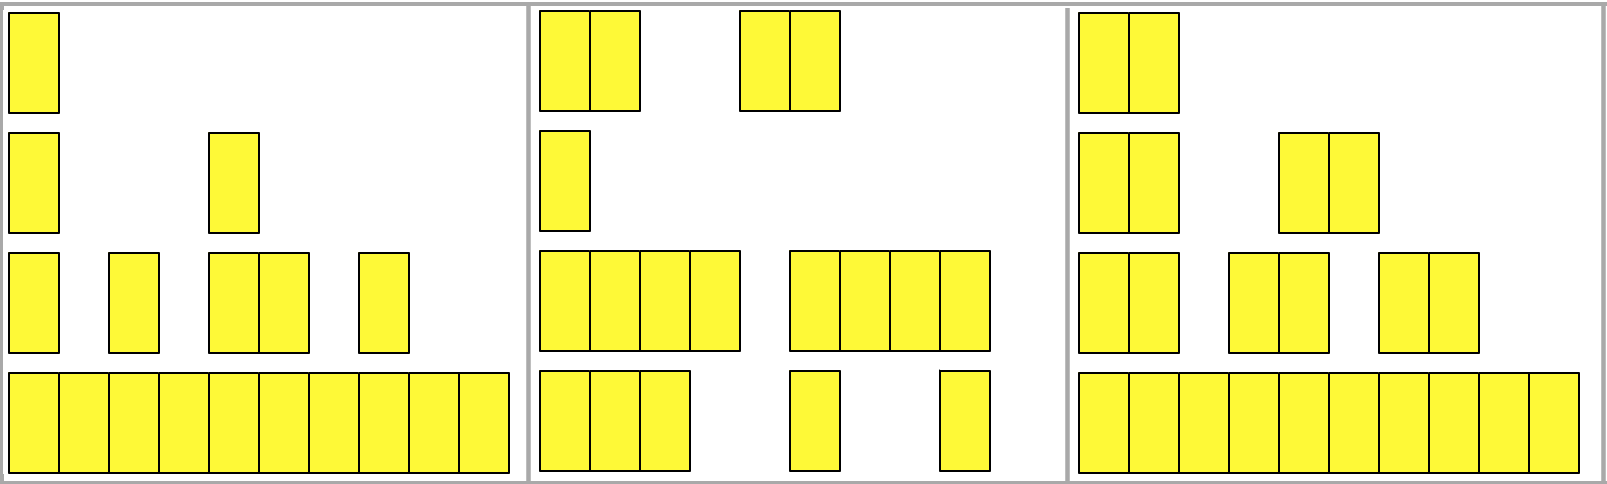
\includegraphics[width = \columnwidth]{./pictures/4_lcs_two/all.png}
\caption{Top results for 4 species partial pattern naming game, with similarity scores from left to right of 16.3, 25, 28.3.}
\end{figure} 

\begin{figure}[h]
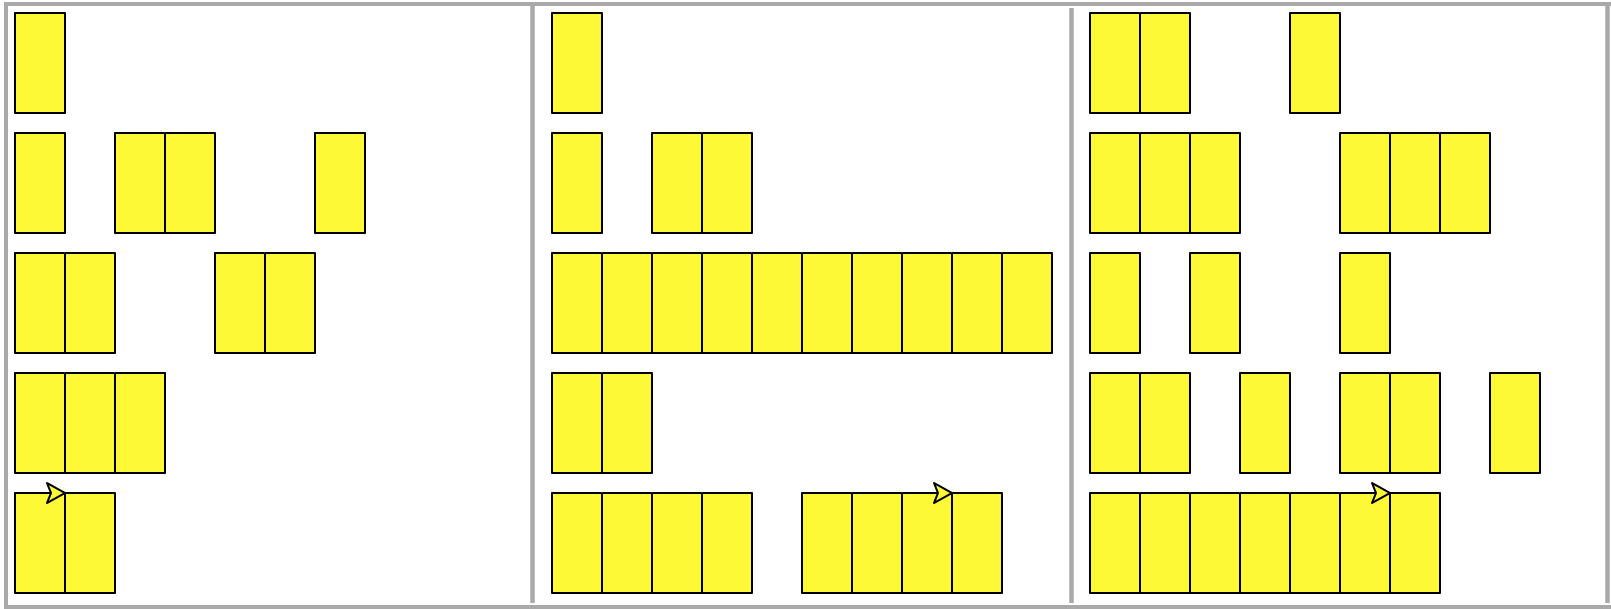
\includegraphics[width = \columnwidth]{./pictures/5_lcs_one/all.png}
\caption{Top results for 5 species full pattern naming game, with similarity scores from left to right of 22.9, 23.1, and 26.3.}
\end{figure} 

\begin{figure}[h]
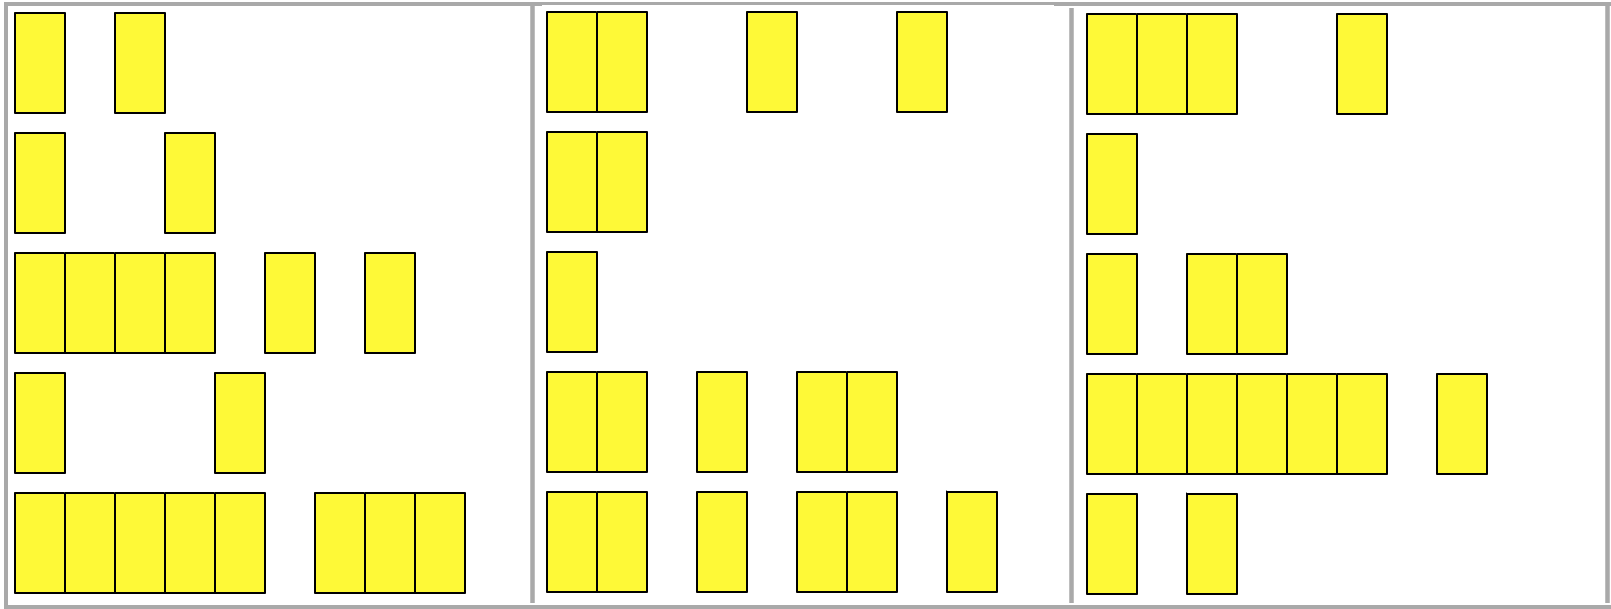
\includegraphics[width = \columnwidth]{./pictures/5_lcs_two/all.png}
\caption{Top results for 5 species partial pattern naming game, with similarity scores from left to right of 24, 25.7, 26.}
\end{figure}   
\subsection{Methods Summary}
In both naming games, fireflies seek to find a flash pattern that is distinctive from the patterns seen in other firefly species, while limiting the number of flashes used to create such differences.
Distinctiveness is measured through one of two similarity scores or by the ability to make the correct decision with respect to partial signal recognition.
We can thus understand the objective function of the simulation as finding the pattern that either minimizes or maximizes (depending on type of naming game) the score function with discounting. 
